\documentclass[../main.tex]{subfiles}
\graphicspath{{\subfix{../img/}}}

\begin{document}
\section{Introduction} \label{sec:introduction}

Sleep-wake cycle in organisms is thought to have evolved due to evolutionary
adaptation to alteration of day and night \cite{suarez-grimaltNeuralArchitectureSleep2021}.
Sleep is characterized by increased periods of inactivity, reduced responses to external stimuli,
tendency for recovery sleep after sleep deprivation, and rapid reversibility, making it
distinct from hibernation or coma
\cite{shaferRegulationDrosophilaSleep2021,andreaniCircadianProgrammingEllipsoid2022,donleaRecurrentCircuitryBalancing2018}.
These behavioral hallmarks of sleep are shared between both vertebrates and invertebrates
inluding files \cite{shaferRegulationDrosophilaSleep2021,andreaniCircadianProgrammingEllipsoid2022},
despite huge variability in the complexity and size of the nervous systems of the organisms.

Although regulation of sleep on the cellular and molecular is not yet fully understood,
across species sleep has been shown to be important for various cellular processes
(e.g. regulation synaptic strength, cellular metabolism, etc.). Furthermore,
poor sleep quality has been linked to numerous health conditions (e.g. diabetes, depression),
as well as negative effects on congitive functions, such as learning, memory,
selective attention and social behavior \cite{shaferRegulationDrosophilaSleep2021,dubowyCircadianRhythmsSleep2017,suarez-grimaltNeuralArchitectureSleep2021}.

Apart from bihavioral similarities, the genetic and molecular mechanisms underlying
sleep are also similar across species \cite{dubowyCircadianRhythmsSleep2017}.
In vertebrates sleep and sleepiness is thought to be linked to large-scale synchronizations in the cortex
resulting in \gls{swa} and reduction of connectivity between brain areas \cite{suarez-grimaltNeuralArchitectureSleep2021,raccugliaNetworkSpecificSynchronizationElectrical2019}.
Interestingly, \gls{swa} with similar characteristics have also been observed in \textit{Drosophila} (fruit files),
where lower degree of synchronization correlates with reduced sleep duration and arousability
threshold, as well as rebound sleep after sleep deprivation
\cite{raccugliaNetworkSpecificSynchronizationElectrical2019}. Moreover, brain-wide
\gls{swa} has been shown to be important for filtering sensory information, thus increasing
arousability threshold during sleep \cite{raccugliaCoherentMultilevelNetwork2022}. These
striking similarities between evolutionary distinct organisms might indicate to existance of
fundamental processes governing sleep regulation \cite{suarez-grimaltNeuralArchitectureSleep2021}.

\textit{Drosophila} is a well-established model to study sleep 
\cite{liuSleepDriveEncoded2016,andreaniCircadianProgrammingEllipsoid2022,shaferRegulationDrosophilaSleep2021,dubowyCircadianRhythmsSleep2017}.
Although its brain is relatively simple (consisting of around 100,000 neurons \cite{donleaRecurrentCircuitryBalancing2018} in comparison to
estimated 86 billion in human brain \cite{herculano-houzelRemarkableNotExtraordinary2012}), \textit{Drosophila} still
shares many similarities in sleep-regulation with vertebrates \cite{liuSleepDriveEncoded2016}, including
mammals \cite{suarez-grimaltNeuralArchitectureSleep2021,dubowyCircadianRhythmsSleep2017} despite long
evolutionary distance (approximately 800 million years \cite{williamsLongReachNAAG2021}).

\textcolor{red}{Short text about circadian and homeostatic regulation + short descriptions
+ mention that R5 is thought to be the core of homeostatic regulation}

The cellular mechanism underlying the switch from tonic to bursting activity in R5 neurons remains poorly understood.
This transition is likely influenced by a combination of factors, including modulation of intracellular ion concentrations,
regulation of ion channel protein expression, and modulation of synaptic strength. Additionally, similar mechanisms
(driven by circadian and homeostatic systems) in neurons that modulate R5 activity may effectively regulate
R5 in a diurnal manner. 
\textcolor{red}{Not much information about ion concentrations and ion channels for Drosophila R5 neurons}

The function of R5 nenetwork has been characterized as analogous to mammalian thalamus
\cite{suarez-grimaltNeuralArchitectureSleep2021,raccugliaNetworkSpecificSynchronizationElectrical2019}.
\gls{tc} relay cells integrate sensory information prior to relaying them to cortex \cite{sampathkumarIntegrationSignalsDifferent2021}.
Similarly, R5 neurons are part of \gls{eb} which integrates sensory information to guide locomotion \cite{yanSubtypeSpecificRolesEllipsoid2023}. 
Furthermore, both R5 and \gls{tc} neurons are filtering sensory information and acting as a
sensory gate that controls shifts between wakefulness and sleep
\cite{raccugliaCoherentMultilevelNetwork2022,gentThalamicDualControl2018}. Both
synchronize electrical patterns and switch from tonic to burst firing (defined as slow alternating transitions between steady and spiking states
\cite{rinzelFormalClassificationBursting1987}) with increasing sleep need, as well as promote transition to sleep
\cite{suarez-grimaltNeuralArchitectureSleep2021, raccugliaNetworkSpecificSynchronizationElectrical2019}.

Although R5 neurons share similar functional characteristits with thalamic neurons,
morphology of neurons in \textit{Drosophila} is significantly different from those in vertebrates
\ref{fig:morphology_drosphila_vs_mammalian}. 
Unlike vertebrates, \textit{Drosophila} neurons have unipolar morphology. Because of this morphology,
synaptic potentials travelling from dendrites to spike initiation zone bypass cell body.
Because of this morphology, the cell body of \textit{Drosophila} neurons is
electronically segregated from other cell regions, suggesting that it is not involved
in synaptic integration \cite{gouwensSignalPropagationDrosophila2009,tuthillLessonsCompartmentalModel2009}.
Furthermore, it has been found that, in contrast to vertebrates, dendrites of
\textit{Drosophila} neurons (slecifically, \gls{kc}) are not solely postsynaptic, but
also form presynaptic active zones \cite{christiansenPresynapsesKenyonCell2011}.

\begin{figure}[!t]
    \centering
    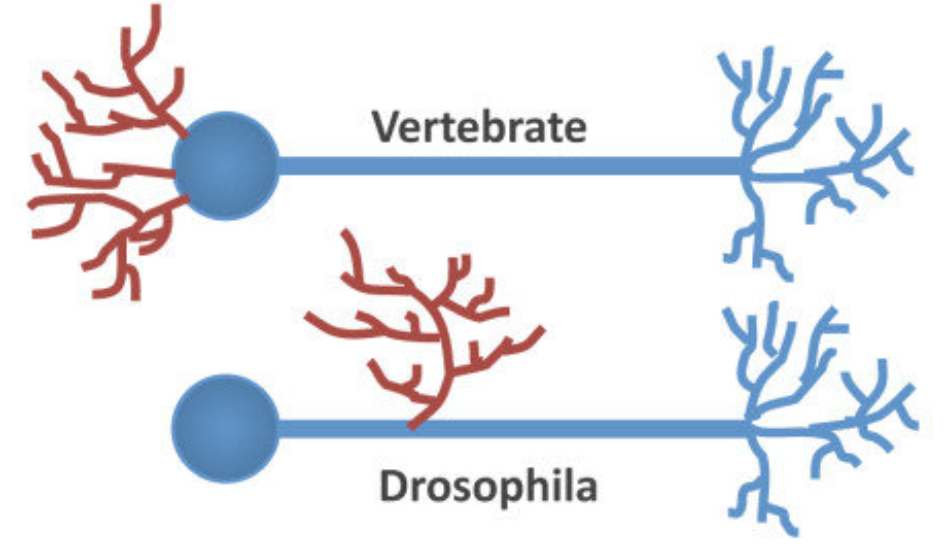
\includegraphics[width=0.55\linewidth]{../img/modelling_r5/examples/drosophila_neuron_morphology.png}
    \caption[Neuron morphology in \textit{Drosophila} and Vertebrates]{
        \textbf{Comparison of neuron morphology in \textit{Drosophila} and Vertebrates.}
        In comparison to vertebrates,
        the neurons in \textit{Drosophila} have unipolar morphology. Therefore synaptic potentials
        travelling from the dendrites (red) to spike initiation zone bypass cell body
        (blue circle). Figure adapted from \cite{spindlerBazookaMediatesSecondary2011}.
    }
    \label{fig:morphology_drosphila_vs_mammalian}
\end{figure}

\color{red}
\begin{itemize}
    \item Posed questions:
    \begin{itemize}
        \item What is the mechanism behind switching between bursting (1Hz) and (low frequency) tonic spikes?
        \item Why is there bursting for T KD? (partial knockdown? Or L type channels?)
        \item Why do we observe increased resting membrane potential with T KD? Ca channels are depolarizing, so
        intuitively reducing depolarizing current should result in hyperpolarization of the membrane
        (there was a modelling paper stating this)
    \end{itemize}
\end{itemize}
\color{black}

%%%%%%%%%%%%%%%%%%%%%%%%%%%%%%%%%%%%%%%%%%%%%%%%%%%%%%%%%%%%%%%%%%%%%%%%%%%%%%%%%%%

\noindent\hrulefill

\noindent\hrulefill

"Bursting can - enhance SNR, facilitate neuropeptide release,
increase reliability of synaptic transmission \cite{vickstromTTypeCalciumChannels2020}
"

"Whether cell-autonomous conductances contribute to sustained rhythmic activities of single R5 neuron remains an open question."
\cite{raccugliaNetworkSpecificSynchronizationElectrical2019} (Raccuglia et al 2019)


\begin{itemize}
    \item Number of neurons and their size in Drosophila (Size: 2-6$\mu m$ in 
    comparison to $10-30\mu m$ for pyramidal cells in rodents) \cite{tuthillLessonsCompartmentalModel2009}.
\end{itemize}

\end{document}